\begin{table}
	\begin{Dtabular}[1.1]{|c|c|c|c|}
		\hline
		$\nu''$&Wellenlänge $\lambda\,$nm&$G\,\text{cm}^{-1}$&$\Delta G\,\text{cm}^{-1}$\\
		\hline
		$25$&$ 509.8 \pm 0.5 $&$ 19617 \pm 4 $&$ 40 \pm 5 $\\
		$26$&$ 510.8 \pm 0.5 $&$ 19577 \pm 4 $&$ 33 \pm 5 $\\
		$27$&$ 511.7 \pm 0.5 $&$ 19543 \pm 4 $&$ 40 \pm 5 $\\
		$28$&$ 512.7 \pm 0.5 $&$ 19504 \pm 4 $&$ 46 \pm 5 $\\
		$29$&$ 513.9 \pm 0.5 $&$ 19458 \pm 4 $&$ 46 \pm 5 $\\
		$30$&$ 515.1 \pm 0.5 $&$ 19412 \pm 4 $&$ 45 \pm 5 $\\
		$31$&$ 516.4 \pm 0.5 $&$ 19366 \pm 4 $&$ 52 \pm 5 $\\
		$32$&$ 517.8 \pm 0.5 $&$ 19314 \pm 4 $&$ 45 \pm 5 $\\
		$33$&$ 519.0 \pm 0.5 $&$ 19269 \pm 4 $&$ 57 \pm 5 $\\
		$34$&$ 520.5 \pm 0.5 $&$ 19212 \pm 4 $&$ 57 \pm 5 $\\
		$35$&$ 522.1 \pm 0.5 $&$ 19155 \pm 4 $&$ 57 \pm 5 $\\
		$36$&$ 523.6 \pm 0.5 $&$ 19098 \pm 4 $&$ 62 \pm 5 $\\
		$37$&$ 525.3 \pm 0.5 $&$ 19036 \pm 4 $&$ 62 \pm 5 $\\
		$38$&$ 527.0 \pm 0.5 $&$ 18974 \pm 4 $&$ 55 \pm 5 $\\
		$39$&$ 528.6 \pm 0.5 $&$ 18919 \pm 4 $&$ 73 \pm 5 $\\
		$40$&$ 530.6 \pm 0.5 $&$ 18846 \pm 4 $&$ 67 \pm 5 $\\
		$41$&$ 532.5 \pm 0.5 $&$ 18779.0 \pm 3.5 $&$ 66 \pm 5 $\\
		$42$&$ 534.4 \pm 0.5 $&$ 18713.3 \pm 3.5 $&$ 71 \pm 5 $\\
		$43$&$ 536.4 \pm 0.5 $&$ 18642.1 \pm 3.5 $&$ 76 \pm 5 $\\
		$44$&$ 538.6 \pm 0.5 $&$ 18566.0 \pm 3.4 $&$ 76 \pm 5 $\\
		$45$&$ 540.8 \pm 0.5 $&$ 18490.4 \pm 3.4 $&$ 75 \pm 5 $\\
		$46$&$ 543.0 \pm 0.5 $&$ 18415.5 \pm 3.4 $&$  85 \pm 5 $\\
		$47$&$ 545.5 \pm 0.5 $&$ 18330.1 \pm 3.4 $& - \\
		\hline
	\end{Dtabular}
	\centering
	\caption[Values of the Transitions by Absorption]{Wavelength and energy of the photons absorbed by the transition of $\nu'=0 \rightarrow \nu'$. There is also the difference of energy $\Delta G$ to the next higher transition.}
	\label{tabAS1}
\end{table}
\begin{figure}[ht]
	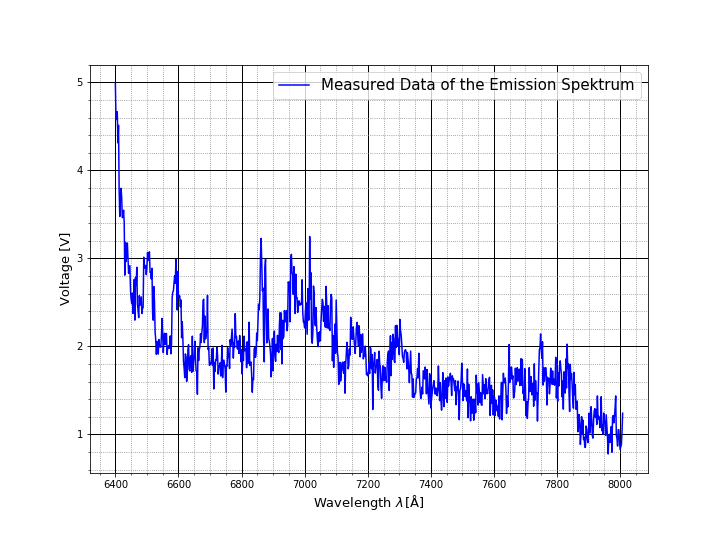
\includegraphics[scale=0.5]{Bild/E1}
	\centering
	\caption{Example of the first Emission Spectrum Measurement.}
\end{figure}
\begin{figure}[ht]
	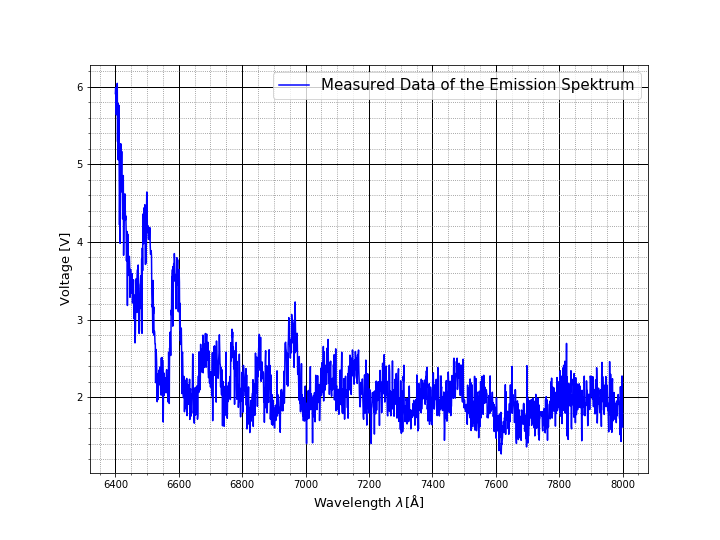
\includegraphics[scale=0.5]{Bild/E2}
	\centering
	\caption{Example of the second Emission Spectrum Measurement.}
\end{figure}
\begin{figure}[ht]
	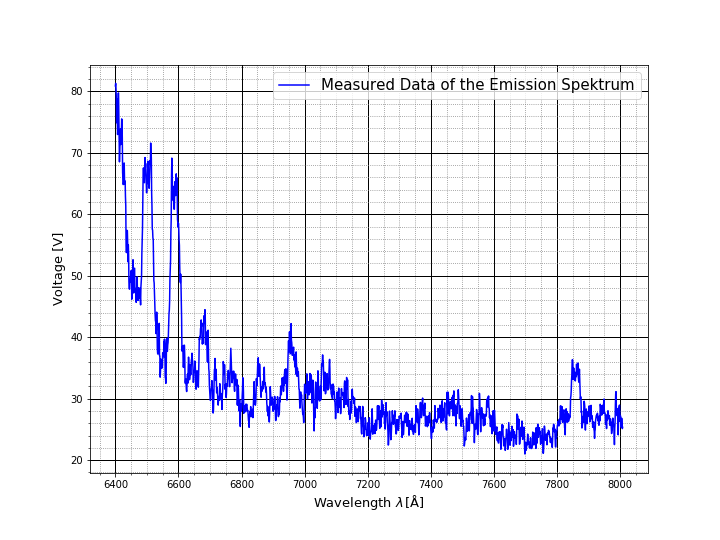
\includegraphics[scale=0.5]{Bild/E4}
	\centering
	\caption{Example of the fourth Emission Spectrum Measurement.}
\end{figure}
\begin{figure}[ht]
	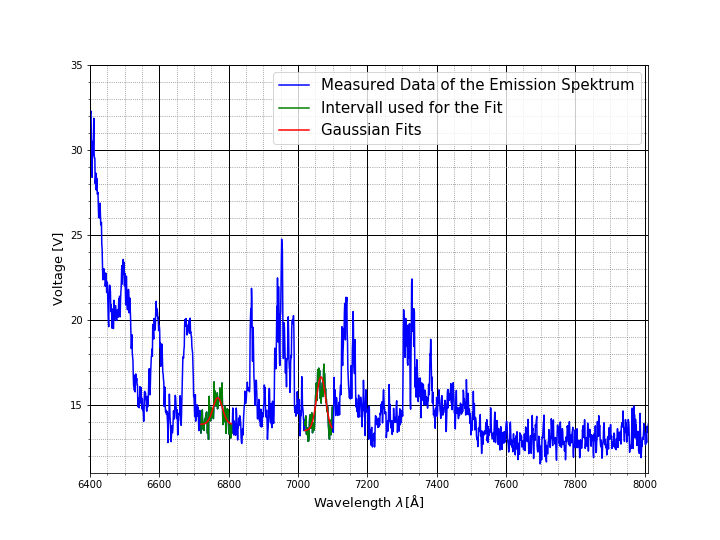
\includegraphics[scale=0.5]{Bild/E3_2}
	\centering
	\caption[Fit of two Peaks in the Emission Spectrum]{Fit of two Peaks in the emission spectrum. In green is the Interval of measured values used for the fit and in red the fit itself.}
	\label{figGausEm}
\end{figure}
\begin{figure}[ht]
	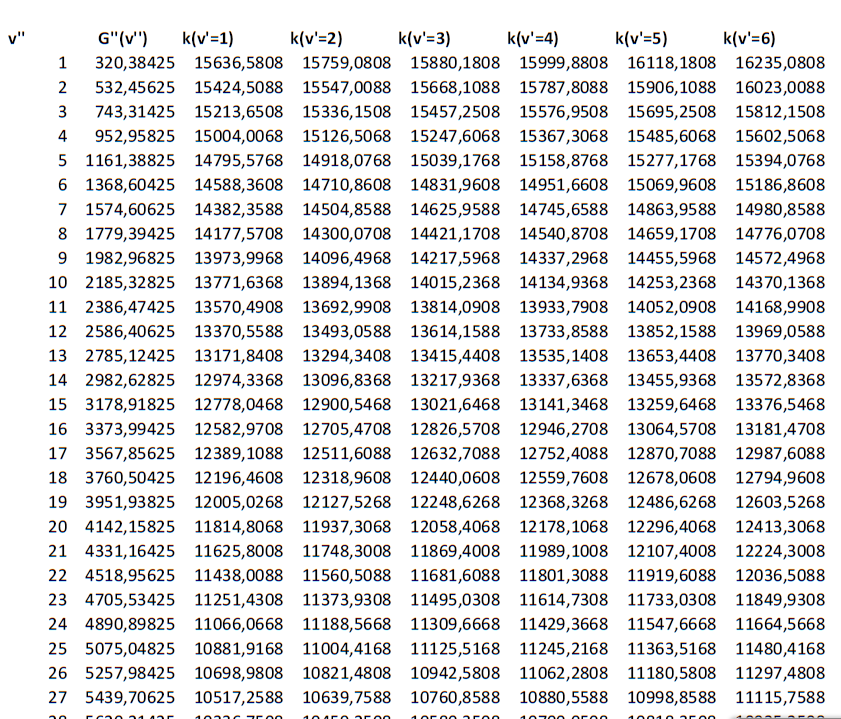
\includegraphics[scale=0.8]{Bild/DATA.png}
	\centering
	\caption[Table with Literature Values]{Figure of the table with literature values used for the analysis of the emission spectrum.\cite{Anleitung}}
\end{figure}